\documentclass[12pt]{article}
\usepackage[left=1cm, right=1cm, top=2cm,bottom=1.5cm]{geometry} 

\usepackage[parfill]{parskip}
\usepackage[utf8]{inputenc}
\usepackage[T2A]{fontenc}
\usepackage[russian]{babel}
\usepackage{enumitem}
\usepackage[normalem]{ulem}
\usepackage{amsfonts, amsmath, amsthm, amssymb, mathtools,xcolor}
\usepackage{blkarray}

\usepackage{tabularx}
\usepackage{hhline}

\usepackage{accents}
\usepackage{fancyhdr}
\pagestyle{fancy}
\renewcommand{\headrulewidth}{1.5pt}
\renewcommand{\footrulewidth}{1pt}

\usepackage{graphicx}
\usepackage[figurename=Рис.]{caption}
\usepackage{subcaption}
\usepackage{float}

%%Наименование папки откуда забирать изображения
\graphicspath{ {./images/} }

%%Изменение формата для ввода доказательства
\renewcommand{\proofname}{$\square$  \nopunct}
\renewcommand\qedsymbol{$\blacksquare$}

%%Изменение отступа на таблицах
\addto\captionsrussian{%
	\renewcommand{\proofname}{$\square$ \nopunct}%
}
%% Римские цифры
\newcommand{\RN}[1]{%
	\textup{\uppercase\expandafter{\romannumeral#1}}%
}

%% Для удобства записи
\newcommand{\MR}{\mathbb{R}}
\newcommand{\MC}{\mathbb{C}}
\newcommand{\MQ}{\mathbb{Q}}
\newcommand{\MN}{\mathbb{N}}
\newcommand{\MZ}{\mathbb{Z}}
\newcommand{\MTB}{\mathbb{T}}
\newcommand{\MTI}{\mathbb{I}}
\newcommand{\MI}{\mathrm{I}}
\newcommand{\MCI}{\mathcal{I}}
\newcommand{\MJ}{\mathrm{J}}
\newcommand{\MH}{\mathrm{H}}
\newcommand{\MT}{\mathrm{T}}
\newcommand{\MU}{\mathcal{U}}
\newcommand{\MV}{\mathcal{V}}
\newcommand{\MB}{\mathcal{B}}
\newcommand{\MF}{\mathcal{F}}
\newcommand{\MW}{\mathcal{W}}
\newcommand{\ML}{\mathcal{L}}
\newcommand{\MP}{\mathcal{P}}
\newcommand{\VN}{\varnothing}
\newcommand{\VE}{\varepsilon}
\newcommand{\dx}{\, dx}
\newcommand{\dy}{\, dy}
\newcommand{\dz}{\, dz}
\newcommand{\dd}{\, d}


\theoremstyle{definition}
\newtheorem{defn}{Опр:}
\newtheorem{rem}{Rm:}
\newtheorem{prop}{Утв.}
\newtheorem{exrc}{Упр.}
\newtheorem{problem}{Задача}
\newtheorem{lemma}{Лемма}
\newtheorem{theorem}{Теорема}
\newtheorem{corollary}{Следствие}

\newenvironment{cusdefn}[1]
{\renewcommand\thedefn{#1}\defn}
{\enddefn}

\DeclareRobustCommand{\divby}{%
	\mathrel{\text{\vbox{\baselineskip.65ex\lineskiplimit0pt\hbox{.}\hbox{.}\hbox{.}}}}%
}
%Короткий минус
\DeclareMathSymbol{\SMN}{\mathbin}{AMSa}{"39}
%Длинная шапка
\newcommand{\overbar}[1]{\mkern 1.5mu\overline{\mkern-1.5mu#1\mkern-1.5mu}\mkern 1.5mu}
%Функция знака
\DeclareMathOperator{\sgn}{sgn}

%Функция ранга
\DeclareMathOperator{\rk}{\text{rk}}
\DeclareMathOperator{\diam}{\text{diam}}


%Обозначение константы
\DeclareMathOperator{\const}{\text{const}}

\DeclareMathOperator{\codim}{\text{codim}}

\DeclareMathOperator*{\dsum}{\displaystyle\sum}
\newcommand{\ddsum}[2]{\displaystyle\sum\limits_{#1}^{#2}}

%Интеграл в большом формате
\DeclareMathOperator{\dint}{\displaystyle\int}
\newcommand{\ddint}[2]{\displaystyle\int\limits_{#1}^{#2}}
\newcommand{\ssum}[1]{\displaystyle \sum\limits_{n=1}^{\infty}{#1}_n}

\newcommand{\smallerrel}[1]{\mathrel{\mathpalette\smallerrelaux{#1}}}
\newcommand{\smallerrelaux}[2]{\raisebox{.1ex}{\scalebox{.75}{$#1#2$}}}

\newcommand{\smallin}{\smallerrel{\in}}
\newcommand{\smallnotin}{\smallerrel{\notin}}

\newcommand*{\medcap}{\mathbin{\scalebox{1.25}{\ensuremath{\cap}}}}%
\newcommand*{\medcup}{\mathbin{\scalebox{1.25}{\ensuremath{\cup}}}}%

\makeatletter
\newcommand{\vast}{\bBigg@{3.5}}
\newcommand{\Vast}{\bBigg@{5}}
\makeatother

%Промежуточное значение для sup\inf, поскольку они имеют разную высоту
\newcommand{\newsup}{\mathop{\smash{\mathrm{sup}}}}
\newcommand{\newinf}{\mathop{\mathrm{inf}\vphantom{\mathrm{sup}}}}

%Скалярное произведение
\newcommand{\inner}[2]{\left\langle #1, #2 \right\rangle }
\newcommand{\linsp}[1]{\left\langle #1 \right\rangle }
\newcommand{\linmer}[2]{\left\langle #1 \vert #2\right\rangle }

%Подпись символов снизу
\newcommand{\ubar}[1]{\underaccent{\bar}{#1}}

%% Шапка для букв сверху
\newcommand{\wte}[1]{\widetilde{#1}}
\newcommand{\wht}[1]{\widehat{#1}}

%%Трансформация Фурье
\newcommand{\fourt}[1]{\mathcal{F}\left(#1\right)}
\newcommand{\ifourt}[1]{\mathcal{F}^{-1}\left(#1\right)}

%%Символ вектора
\newcommand{\vecm}[1]{\overrightarrow{#1\,}}

%%Пространстов матриц
\newcommand{\matsq}[1]{\operatorname{Mat}_{#1}}
\newcommand{\mat}[2]{\operatorname{Mat}_{#1, #2}}

%Оператор для действ и мнимых чисел
\DeclareMathOperator{\IM}{\operatorname{Im}}
\DeclareMathOperator{\RE}{\operatorname{Re}}
\DeclareMathOperator{\li}{\operatorname{li}}
\DeclareMathOperator{\GL}{\operatorname{GL}}
\DeclareMathOperator{\SL}{\operatorname{SL}}



%%Взятие в скобки, модули и норму
\newcommand{\parfit}[1]{\left( #1 \right)}
\newcommand{\modfit}[1]{\left| #1 \right|}
\newcommand{\sqparfit}[1]{\left\{ #1 \right\}}
\newcommand{\normfit}[1]{\left\| #1 \right\|}

%%Функция для обозначения равномерной сходимости по множеству
\newcommand{\uconv}[1]{\overset{#1}{\rightrightarrows}}
\newcommand{\uconvm}[2]{\overset{#1}{\underset{#2}{\rightrightarrows}}}


%%Функция для обозначения нижнего и верхнего интегралов
\def\upint{\mathchoice%
	{\mkern13mu\overline{\vphantom{\intop}\mkern7mu}\mkern-20mu}%
	{\mkern7mu\overline{\vphantom{\intop}\mkern7mu}\mkern-14mu}%
	{\mkern7mu\overline{\vphantom{\intop}\mkern7mu}\mkern-14mu}%
	{\mkern7mu\overline{\vphantom{\intop}\mkern7mu}\mkern-14mu}%
	\int}
\def\lowint{\mkern3mu\underline{\vphantom{\intop}\mkern7mu}\mkern-10mu\int}

%%След матрицы
\DeclareMathOperator*{\tr}{tr}

\makeatletter
\renewcommand*\env@matrix[1][*\c@MaxMatrixCols c]{%
	\hskip -\arraycolsep
	\let\@ifnextchar\new@ifnextchar
	\array{#1}}
\makeatother


%% Переопределение функции хи, чтобы выглядела более приятно
\makeatletter
\@ifdefinable\@latex@chi{\let\@latex@chi\chi}
\renewcommand*\chi{{\@latex@chi\smash[t]{\mathstrut}}} % want only bottom half of \mathstrut
\makeatletter

\begin{document}
\lhead{Алгебра-\RN{1}}
\chead{Тимашев Д.А.}
\rhead{Лекция - 11}
\section*{Основные алгебраические структуры}
\begin{defn}
	\uwave{Бинарная операция} на множестве $M$ - это отображение из множества пар $M \times M$ в само множество $M$: 
	$$
		M\times M \to M \colon (a,b) \mapsto a\circ b
	$$
	называемая обычно \uwave{умножением}, где $a\circ b$ называется \uwave{произведением элементов}.
\end{defn}
\begin{rem}
	По определению любой паре $(a,b) \in M \times M$ должен сопоставляться элемент множества $M$ и причем ровно один.
\end{rem}
Если $|M| = m$, то $|M\times M| = m^2 \Rightarrow$ всего $m^{m^2}$ бинарных операций существует.

\begin{defn}
	\uwave{Полугруппой} $(S,\circ)$ называется множество $S$ с бинарной операцией $\circ$, удовлетворяющей требованию ассоциативности:
	$$
		\forall a,b,c \in S,\, a \circ (b\circ c) = (a\circ b)\circ c
	$$
\end{defn}

\textbf{Примеры полугрупп}:
\begin{enumerate}[label=\arabic*)]
	\item $(\MN, +)$;
	\item $(\MN, \times)$;
	\item Пусть $S$ - множество всех отображений $M \to M$, пусть $\psi, \varphi \in S$, композиция $\varphi \circ \psi$ ассоциативна, тогда $(S,\circ)$ - полугруппа;
	\item Пусть $S = M$, где $M$ - любое множество, определим композицию: $\forall a,b \in S,\, a \circ b = a$, тогда такая операция ассоциативна. Действительно $\forall a,b,c \in S$:
	$$
		a \circ (b \circ c) = a \circ b = a
	$$
	$$
		(a \circ b) \circ c = a \circ c = a
	$$
	\item Пусть $S = M$, где $M$ - любое множество, определим композицию: $\forall a,b \in S,\, a \circ b = U \in M$, тогда такая операция ассоциативна. Действительно $\forall a,b,c \in S$:
	$$
		a \circ (b \circ c) = a \circ U = U
	$$
	$$
		(a \circ b) \circ c = U \circ c = U
	$$
	\item Пусть $S = \MN, \, \forall a,b \in S, \, a \circ b = a^b$, тогда такая операция не ассоциативна. Действительно:
	$$
		2 \circ ( 1 \circ 3 ) = 2 \circ 1^3  = 2 \circ 1 = 2^1 = 2
	$$
	$$
		(2 \circ 1)\circ 3 = 2^1 \circ 3 = 2^3 = 8
	$$
\end{enumerate}

\begin{defn}
	Полугруппа $(S,\circ)$ называется \uwave{моноидом}, если в $S$ существует \uwave{единица} или \uwave{нейтральный элемент}, то есть такой элемент $e \in S$:
	$$
		\forall a \in S,\, a \circ e = e\circ a = a
	$$
\end{defn}


\textbf{Примеры моноидов}:
\begin{enumerate}[label=\arabic*)]
	\item $(\MN \cup \{0\}, +), \, e = 0$;
	\item $(\MN, \times), \, e = 1$;
\end{enumerate}

\subsection*{Группы}
\begin{defn}
	\uwave{Группа} - это множество $G$, на котором задана \uwave{бинарная операция} $\circ \colon G \times G \to G$, которая должна удовлетворять свойствам, называемыми \uline{аксиомами группы}:
	\begin{enumerate}[label=\arabic*)]
		\item \textbf{Ассоциативность}: 
		$$
			\forall a,b,c \in G,\, (a \circ b)\circ c = a\circ (b \circ c)
		$$
		\item \textbf{Существование нейтрального элемента}: 
		$$	
			\exists \, e \in G \colon \forall g \in G, \, g \circ e = e \circ g = g
		$$
		где $e$ - \uwave{нейтральный элемент} или ещё его называют \uwave{единицей} в группе $G$;
		\item \textbf{Существование обратного элемента}:
		$$
			\forall g \in G, \, \exists \, h \in G \colon g \circ h = h \circ g = e	
		$$
		где $h$ - \uwave{обратный элемент} к элементу $g$;
	\end{enumerate}
\end{defn}

\subsection*{Простейшие следствия аксиом группы}
\begin{prop}
	Нейтральный элемент единственен:
	$$
		\exists! \, e \in G \colon \forall g \in G, \, g \circ e = e \circ g = g
	$$
\end{prop}
\begin{proof}
	Пусть существует две единицы $e, e' \in S$, тогда:
	$$
		e\circ e' = e' \wedge e \circ e' = e \Rightarrow e' = e
	$$	
\end{proof}
\begin{prop}
	Обратный элемент единственен:
	$$
		\forall g \in G, \, \exists! \, h \in G \colon g \circ h = h \circ g = e
	$$
\end{prop}
\begin{proof}
	Пусть существуют два обратных элемента для $g \in S \colon h, h' \in S$, тогда:
	$$
		h = e\circ h = (h' \circ g) \circ h  = h' \circ (g \circ h)	= h' \circ e = h'
	$$
\end{proof}
\textbf{\uline{Обозначение}}: обратный элемент для элемента $g \in G$ обозначается как $g^{-1}$.

\begin{defn}
	Группа $(G, \circ)$ называется \uwave{коммутативной} или \uwave{Абелевой}, если выполнена ещё одна аксиома:
	\begin{enumerate}[label=\arabic*)]
		\setcounter{enumi}{3}
		\item \textbf{Аксиома коммутативности}:
			$$
				\forall a,b \in G, \, a \circ b = b \circ a
			$$
	\end{enumerate}
\end{defn}

Отметим, что операция $\circ$ может быть аддитивной или мультипликативной. В аддитивном случае $\circ \equiv +$, в мультипликативном $\circ \equiv \cdot$. В аддитивном случае $e = 0$, в мультипликативном $e = 1$. Обратный элемент в аддитивном случае обозначается как $-a$, в мультипликативном как $a^{-1}$.

\newpage
\textbf{Примеры групп}:
\begin{enumerate}[label=\arabic*)]
	\item $(\MN, \times), \, e = 1$ - не будет группой, поскольку нарушается $3$-ья аксиома;
	\item $(S_n, \circ)$ - множество подстановок $S_n$ степени $n$ с операцией композиции $\Rightarrow$ группа. Мы доказывали это, когда разбирали подстановки. Но эта группа - неабелева, нет коммутативности композиции;
	\item $(\MR^n, +)$ - множество строк или столбцов в $\MR^n$ с операцией сложения строк или столбцов: 
	$$
		(a_1 , \dotsc, a_n) + (b_1, \dotsc, b_n) = (a_1 + b_1,\dotsc, a_n + b_n)
	$$
	является абелевой группой, потому что оперция сложения строк - коммутативна;
	\item $(\MZ,+)$ - абелева группа: сложение целых чисел коммутативно и ассоциативно, $\forall a \in \MN, \, -a$ это обратный элемент;
	
	\item $(\MQ_+, \times)$ - абелева группа: умножение коммутативно, ассоциативно, еденица - число $1$, обратный элемент к $a \in \MQ_{+}$ это $\tfrac{1}{a} \in \MQ_{+}$;
	
	\item $(\MQ \setminus \{0\}), \times)$ - абелева группа. Для $0$ не существует обратного элемента;
	
	\item $(\MR, +), \, (\MR\setminus\{0\}, \times)$ - абелевы группы;
	
	\item $(\MZ_n,+)$ - группа вчетов по модулю $n$ (будут обсуждаться далее) также абелева. Нейтральный элемент - $\overline{0}$. Обратный элемент к вычету $\overline{k}$ это вычет $\overline{n-k}$. Сложение вычетов ассоциативно и коммутативно. Заметим, что эта группа - конечна;
	
	\item $(\mat{n}{n}, \, \times)$ - является моноидом, но не группой. Единица - единичная матрица. Но у матриц с нулевым определителем не существует обратного элемента;
	
	\item $(\GL_n(\MR),\times), \, \GL_n(\MR) = \{A \in \mat{n}{n} \colon |A| \neq 0\}$ - \uwave{общая линейная группа} это квадратные невырожденные матрицы $n \times n$ с операцией умножения $\Rightarrow$ группа. Единица - единичная матрица. Обратная матрица определена для всех элементов. Умножение матриц ассоциативно, но не коммутативно, следовательно группа неабелева;
	
	\item $(\SL_n(\MR), \times), \, \SL_n(\MR) = \{A \in \mat{n}{n} \colon |A| = 1\}$ - также будет группой с анологичными свойствами, как у $(\GL_n(\MR),\times)$;
\end{enumerate}

\begin{defn}
	 Множество подстановок $S_n$ степени $n$ с операцией композиции называется \uwave{симметрической группой}.
\end{defn}
\begin{defn}
	Множество квадратных матриц размера $n\times n$ у которых определитель не равен нулю называется \uwave{общей линейной группой} относительно операции умножения и обозначается:
	$$
		\GL_n(\MR) = \{A \in \mat{n}{n} \colon |A| \neq 0\}
	$$
	также она называется \uwave{полной матричной группой}.
\end{defn}
\begin{defn}
	Множество квадратных матриц размера $n\times n$ у которых определитель равен единице называется \uwave{специальной линейной группой} относительно операции умножения и обозначается:
	$$
		\SL_n(\MR) = \{A \in \mat{n}{n} \colon |A| = 1\}
	$$
\end{defn}

\begin{rem}
	В абелевых группах операция часто называется сложением и обозначается соответственно.
\end{rem}

Множество с бинарными операциями $\supseteq$ полугруппы $\supseteq$ моноиды $\supseteq$ группы $\supseteq$ абелевы группы.

\newpage
\begin{exrc}
	Пусть $G$ - группа и $\forall g \in G, \, gg = e$. Доказать, что $G$ - абелева.
\end{exrc}
\begin{proof}
	$$
		\forall a, b \in G, \, abab = e = baba \Rightarrow aba = babab = b(abab) = b \Rightarrow (aa)ba = ba = ab 
	$$
\end{proof}

\begin{center}
	\begin{tabular}{ | m{5cm} || m{6cm}| m{7cm} | } 
		\hline
		\textbf{Терминология} & \textbf{Мультипликативная} & \textbf{Аддитивная}\\ [0.5ex]
		\hline\hline
		\textbf{Операция в группе} & Умножение: $a\circ b$ или $a{\cdot}b$ & Сложение: $a + b$ \\ 
		\hline
		\textbf{Нейтральный элемент} & Единица: $e$ или $1$ & Нуль: $0$\\ 
		\hline
		& Обратный элемент: $g^{-1}$ & Противоположный элемент: $-g$\\
		\hline
		& Степень: $g^n, \, n \in \MZ$ & Целое кратное: $n{\cdot}g, \, n \in \MZ$ \\[0.5ex]
		& $n > 0$: $g^n = \underbrace{g{\cdot}\dotsc{\cdot}g}_{n}, \, n \in \MN$ 
		& $n > 0$: $n{\cdot}g = \underbrace{g + \dotsc + g}_{n}, \, n \in \MZ$ \\[4ex]
		& $n < 0$: $g^n = \underbrace{g^{-1}{\cdot}\dotsc{\cdot}g^{-1}}_{|n|}, \, n \in \MZ$ 
		& $n < 0$: $n{\cdot}g = \underbrace{(-g) + \dotsc + (-g)}_{|n|}, \, n \in \MZ$ \\[4ex]
		& $n = 0$: $g^0 = e$ & $n = 0$: $0{\cdot}g = 0$ \\[0.5ex]
		\hline
	\end{tabular}
\end{center}

\subsection*{Подгруппы}

\begin{defn}
	Пусть $G$ - группа. Подмножество $H\subseteq G$ называется \uwave{подгруппой}, если:
	\begin{enumerate}[label=\arabic*)]
		\item $H \neq \VN$;
		\item $\forall a,b \in H,\, a {\cdot}b \in H$;
		\item $\forall a \in H, \, a^{-1} \in H$;
	\end{enumerate}
	то есть это непустое подмножество, которое замкнуто относительно операций перемножения элементов и взятия обратного.
\end{defn}

\begin{prop}
	Единица всегда принадлежит подгруппе: $e \in H \subseteq G$.
\end{prop}
\begin{proof}
	Так как $H \neq \VN$, то 
	$$
		\exists \, h \in H \Rightarrow \exists \, h^{-1} \in H \Rightarrow h\cdot h^{-1} = e \in H
	$$
\end{proof}
\begin{prop}
	Подгруппа сама является группой относительно той же операции $\circ$ в $G$, ограниченной на $H$.
\end{prop}
\begin{proof}
	Ограничивая $\circ$ на подмножество $H$, по свойству $2)$ мы не будем выходить за пределы $H$:
	$$
		\forall a,b \in H \Rightarrow a{\circ_H}b \in H
	$$
	Ассоциативность вытекает из ассоциативности на большем множестве, единичный элемент содержится по утверждению выше, по свойству $3)$ каждый обратный элемент также существует в $H \Rightarrow$ все три аксиомы группы выполнены.
\end{proof}

\textbf{Примеры подгрупп}:
\begin{enumerate}[label=\arabic*)]
	\item \uwave{Множество четных подстановок} $A_n \subset S_n$ это подгруппа, так как по свойствам знака подстановок, при перемножении четных подстановок снова получим четную подстановк, обратная к четной подстановке - четная, тождественная подстановка - четная $\Rightarrow$ непустое множество;
	
	\item \uwave{Множество нечетных подстановок} $S_n \setminus A_n$ не является подгруппой, поскольку произведение любых двух нечетных подстановок будет четной подстановкой $\Rightarrow$ нарушается второе условие;
	
	\item $(\MZ,+)$, $H = \{-1,1\}$ - не является подгруппой, поскольку не содержит $0$, но является группо относительно умножения;
\end{enumerate}

\begin{defn}
	Множество четных подстановок $A_n \subset S_n$ называется \uwave{знакопеременной группой степени} $n$.
\end{defn}

\begin{prop}
	Верно следующее:
	$$
		\forall a,b \in H, \, a{\cdot}b^{-1} \in H \Leftrightarrow 
		\begin{cases}
			\forall a,b \in H, \, a{\cdot}b \in H \\
			\forall a \in H, \, a^{-1} \in H
		\end{cases}
	$$
\end{prop}
\begin{proof}\hfill\\
	$(\Rightarrow)$ $\forall a,b \in H, \, a{\cdot}b^{-1} \in H \Rightarrow a{\cdot}a^{-1} = e \in H$, тогда: $e{\cdot}b^{-1} = b^{-1} \in H$, $a{\cdot}(b^{-1})^{-1} = a{\cdot}b \in H$.
	
	$(\Leftarrow)$ $\forall a,b \in H, \, a{\cdot}b \in H, \, b^{-1} \in H \Rightarrow a{\cdot}b^{-1} \in H$.
\end{proof}

\begin{rem}
	В любой группе $G$ всегда есть подгруппы $H = \{e\}, \, H = G$ - \uwave{несобственные подгруппы}. Остальные подгруппы - \uwave{собственные}.
\end{rem}

\subsection*{Кольцо}

\begin{defn}
	\uwave{Кольцо} $(K,+,\times)$ - это множество $K$ с двумя бинарными операциями - сложением и умножением, которые удовлетворяют свойствам, называемыми \uline{аксиомами кольца}:
	\begin{enumerate}[label=\arabic*)]
		\item \textbf{Коммутативность сложения}:
		$$
			\forall a,b \in K, \, a + b = b + a
		$$
		\item \textbf{Ассоциативность сложения}:
		$$
			\forall a,b,c \in K, \, a + (b + c) = (a + b) + c
		$$
		\item \textbf{Существование нулевого элемента}:
		$$
			\exists \, 0 \in K \colon \forall a \in K, \, 0 + a = a
		$$
		\item \textbf{Существование противоположного элемента}:
		$$
			\forall a \in K, \, \exists \, b \in K \colon a + b =0
		$$
		\textbf{\uline{Обозначение}}: $b = -a$
		\item \textbf{Дистрибутивность умножения относительно сложения} (левая):
		$$
			\forall a,b,c \in K, \, a{\cdot}(b + c) = a{\cdot}b + a{\cdot}c
		$$
		\item \textbf{Дистрибутивность умножения относительно сложения} (правая):
		$$
			\forall a,b,c \in K, \, (b + c){\cdot}a = b{\cdot}a + c{\cdot}a
		$$
	\end{enumerate}
	Свойства $1) - 4)$ для множества $K$ относительно операции сложения дают структуру абелевой группы, то есть: $(K,+)$ - абелева группа. Такая группа называется \uwave{аддитивной группой кольца} $K$.
\end{defn}

\begin{rem}
	Правая дистрибутивность не следует из левой и наобоорот, потому что про умножение нет предположения о коммутативности.
\end{rem}

\subsection*{Классы колец}

\begin{defn}
	Кольцо $(K, +,\times)$ называется \uwave{коммутативным}, если $\forall a,b \in K, \, a{\cdot}b = b{\cdot}a$.
\end{defn}

\begin{defn}
	Кольцо $(K, +,\times)$ называется \uwave{ассоциативным}, если $\forall a,b,c \in K, \, a{\cdot}(b{\cdot}c) = (a{\cdot}b){\cdot}a$.
\end{defn}

\begin{defn}
	Кольцо $(K, +,\times)$ называется \uwave{кольцом с единицей}, если $\exists \, 1 \in K \colon \forall a \in K, \, 1{\cdot}a = a{\cdot}1 = a$.
\end{defn}

Существуют и другие классы колец, которые мы пока затрагивать не будем.

\textbf{Примеры колец}:
\begin{enumerate}[label=\arabic*)]
	\item $(\MZ, +, \times)$ - коммутативное, ассоциативное кольцо с единицей;
	\item $(\mat{n}{n}, +,\times)$ - некоммутативное, ассоциативное кольцо с единицей;
	\item $K = \{\textbf{геом. векторы в пространстве}\}$ с операциями сложения векторов и векторного произведения, где $\forall a,b \in K$ векторное произведение $a{\cdot}b$ это вектор, перпендикулярный плоскости натянутой на $a,b$, длина которого равна площади параллелограмма построенного на этих векторах.
	\begin{figure}[H]
		\centering
		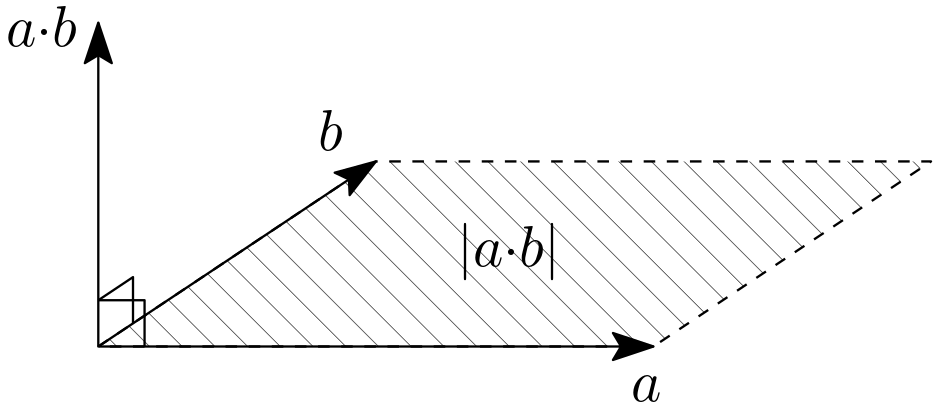
\includegraphics[width=0.4\textwidth]{AL1L11_1.png}
		\caption{Векторное произведение}
		\label{11_1}
	\end{figure}
	Это будет некоммутативное, неассоциативное кольцо без единциы (поскольку любой вектор, умноженный сам на себя даст $0$);
	\item $(\MZ,+,\times)$ - коммутативное, ассоциативное кольцо;
	\item $(\MQ,+,\times)$ - коммутативное, ассоциативное кольцо;
	\item $(\MR, +,\times)$ - коммутативное, ассоциативное кольцо;
	\item $(\MZ_n, +, \times)$ - конечное, коммутативное кольцо вычетов;
	\item $(\MF(M,\MR), +,\times)$ - кольцо функций, где $M$ - произвольное множество, $f \colon M \to \MR$. Рассмотрим все такие функции $\MF(M,\MR) = \{f\colon M \to \MR\}$ и введем на этом множестве бинарные операции:
	$$
		(f_1 + f_2)(m) = f_1(m) + f_2(m), \, \forall m \in M
	$$
	$$
		(f_1{\cdot}f_2)(m) = f_1(m){\cdot}f_2(m), \, \forall m \in M
	$$
	Множество функций с операцией $+$ - абелева группа, умножение функций ассоциативно и обладает единицей ($f\equiv 1)$, умножение коммутативно поскольку коммутативно умножение действительных чисел. Следовательно, это коммутативное, ассоциативное кольцо;
\end{enumerate}
\newpage
\subsection*{Простейшие следствия аксиом кольца}

\begin{prop}
	Нулевой элемент единственен:
	$$
		\exists! \, 0 \in K \colon \forall a \in K, \,  0 + a = a
	$$
\end{prop}
\begin{proof}
	Следует напрямую из такого же свойства для группы. В качестве упражнения, пусть $0, 0' \in K$ - два нулевых элемента, тогда:
	$$
		0 = 0 + 0' = 0' + 0 = 0'
	$$
\end{proof}

\begin{prop}
	Противоположный элемент единственен для каждого $a\in K$:
	$$
		\forall a \in K, \, \exists !\, b \in K \colon a + b = 0
	$$
\end{prop}
\begin{proof}
	Аналогично следует напрямую из свойства для группы. Пусть $b, b' \in K$ - два противоположных элемента $\forall a \in K$, тогда:
	$$
		b  = b + 0 =  b + (a + b') = (b + a) + b' = 0 + b' = b'
	$$
\end{proof}
\begin{rem}
	Всякое кольцо является абелевой группой по сложению и там мы уже доказывали свойства выше $\Rightarrow$ доказано.
\end{rem}

\begin{prop}
	Единичный элемент для кольца с единицей - единственен:
	$$
		\exists! \, 1 \in K \colon \forall a \in K, \, a{\cdot}1 = 1{\cdot}a = a
	$$
\end{prop}
\begin{proof}
	Пусть существует две единицы $1,1' \in K$, тогда:
	$$
		1 = 1{\cdot}1' = 1'{\cdot}1 = 1'
	$$
\end{proof}

\begin{prop}
	$\forall a \in K, \, 0{\cdot}a = a{\cdot}0 = 0$.
\end{prop}
\begin{proof}
	$$
		\forall a \in K, \, 0{\cdot}a = (0 + 0){\cdot}a = 0{\cdot}a + 0{\cdot}a \Rightarrow 0{\cdot}a + (-(0{\cdot}a)) = 0{\cdot}a + 0{\cdot}a + (-(0{\cdot}a)) \Rightarrow 0 = 0{\cdot}a
	$$
	$$
		\forall a \in K, \, a{\cdot}0 = a{\cdot}(0 + 0) = a{\cdot}0 + a{\cdot}0 \Rightarrow a{\cdot}0 + (-(a{\cdot}0)) = a{\cdot}0 + a{\cdot}0 + (-(a{\cdot}0)) \Rightarrow 0 = a{\cdot}0 
	$$
\end{proof}
\begin{prop}
	В кольце с единицей будет верно: $\forall a \in K, \, (-1){\cdot}a =a{\cdot}(-1)= -a$.
\end{prop}
\begin{proof}
	$$
		\forall a\in K, \, a + (-1){\cdot}a = 1{\cdot}a + (-1){\cdot}a = (1 + (-1)){\cdot}a = 0{\cdot}a = 0 \Rightarrow (-1){\cdot}a = -a
	$$
	$$
		\forall a\in K, \, a + a{\cdot}(-1) = a{\cdot}1 + a{\cdot}(-1) = a{\cdot}(1 + (-1)) = a{\cdot}0 = 0 \Rightarrow a{\cdot}(-1) = -a
	$$
\end{proof}
Будем рассматривать далее только\textbf{ ассоциативные кольца с единицей}.

\subsection*{Обратимость элементов}
\begin{defn}
	Пусть $K$ - кольцо (ассоциативное с единицей). Элемент $a\in K$ назовем \uwave{обратимым}, если:
	$$
		\exists \, b \in K \colon a{\cdot}b = b{\cdot}a = 1
	$$
	элемент $b$ называется \uwave{обратным элементом} к элементу $a$ и обозначается $b = a^{-1}$. 
\end{defn}
\begin{prop}
	Обратный элемент для обратимого элемента $a$ - единственен:
	$$
		\exists! \, b \in K \colon a{\cdot}b = b{\cdot}a = 1
	$$
\end{prop}
\begin{proof}
	Пусть $b,b' \in K$ - обратные элементы для $a \in K$, тогда:
	$$
		b = b{\cdot}1 = b{\cdot}(a{\cdot}b') = (b{\cdot}a){\cdot}b' = 1{\cdot}b' = b'
	$$
\end{proof}

\begin{rem}
	Заметим, что не у каждого элемента есть обратный, тогда как в группе у каждого.
\end{rem}

\begin{prop}
	Если $|K| > 1$, то $0$ - необратим.
\end{prop}

\begin{proof}
	Покажем сначала, что $1 \neq 0$, иначе:
	$$
		\forall a \in K, \, a = a{\cdot}1 = a{\cdot}0 = 0 \Rightarrow |K| = 1
	$$
	получили противоречие $\Rightarrow 1 \neq 0$, тогда:
	$$
		\forall b \in K, \, 0{\cdot}b = b{\cdot}0 = 0 \neq 1 \Rightarrow \nexists \, 0^{-1}
	$$
\end{proof}

\begin{rem}
	Если $|K| =1$, то ноль будет обратимым, поскольку умножением самого на себя даст сам себя.
\end{rem}

\begin{prop}
	Положим $K^{\times} = \{a\in K \colon \exists \, b \in K \colon a{\cdot}b = b{\cdot}a = 1\}$. Докажем следующее:
	\begin{enumerate}[label=\arabic*)]
		\item $\forall a,b \in K^{\times}, \, a{\cdot}b \in K^{\times}$;
		\item $(K^{\times}, \times)$ - группа, называемая \uwave{мультипликативной группой} кольца $K$;
	\end{enumerate}
\end{prop}

\begin{defn}
	\uwave{Мультипликативная группа} кольца $K$ это множество его обратимых элементов с операцией умножения.
\end{defn}

\begin{proof}\hfill
	\begin{enumerate}[label=\arabic*)]
		\item Докажем, что $(a{\cdot}b)^{-1} = b^{-1}{\cdot}a^{-1} \Rightarrow (a{\cdot}b)^{-1} \in K^{\times}$: 
		$$
			(a{\cdot}b){\cdot}(b^{-1}{\cdot}a^{-1}) = a{\cdot}(b{\cdot}b^{-1}){\cdot}a^{-1} = a{\cdot}1{\cdot}a^{-1} = a{\cdot}a^{-1} = 1 
		$$
		$$
			(b^{-1}{\cdot}a^{-1}){\cdot}(a{\cdot}b) = b^{-1}{\cdot}(a^{-1}{\cdot}a){\cdot}b = b^{-1}{\cdot}1{\cdot}b = b^{-1}{\cdot}b = 1
		$$
		Перестановку скобок во всех таких доказательствах мы делаем по ассоциативности операций;
		\item $1 \in K^{\times} \Rightarrow K^{\times} \neq \VN$, множество обратимых элементов замкнуто относительно умножения $a{\cdot}b \in K^{\times}$. Если $a \in K^{\times}$ - обратим, то $a^{-1} \in K^{\times}$ и $(a^{-1})^{-1} = a$. Следовательно, это группа;
	\end{enumerate}
\end{proof}

\newpage

\textbf{Примеры мультипликативных группы кольца}:
\begin{enumerate}[label=\arabic*)]
	\item $\MZ^{\times} = \{-1,1\}$ - так как для всех остальных элементов обратные будут дробями;
	\item $\mat{n}{n}^{\times} = \GL_n(\MR) = \{A \colon \rk{A} = n\} = \{A \colon \det{A} \neq 0\}$;
	\item $\MQ^{\times} = \MQ \setminus \{0\}$;
	\item $\MR^{\times} = \MR \setminus \{0\}$;
	\item $\MF(M,\MR)^{\times} = \{f \colon f(m) \neq 0, \, \forall m \in M\}$;
	\item $\MZ_n^{\times} = \{\overline{k} \in \MZ_n \colon (k,n) = 1\}$ по теореме из курса теории чисел;
\end{enumerate}

\begin{defn}
	Элемент $a \in K, \, a \neq 0$ называется \uwave{левым делителем нуля}, если: 
	$$
		\exists \, b \in K, \, b \neq 0 \colon a{\cdot} b =0
	$$
\end{defn}
\begin{defn}
	Элемент $a \in K, \, a \neq 0$ называется \uwave{правым делителем нуля}, если: 
	$$
		\exists \, b \in K, \, b \neq 0 \colon b{\cdot}a =0
	$$
\end{defn}
\begin{rem}
	Левые и правые делители бывают потому что умножение, вообще говоря, некоммутативно. Заметим, что к левому делителю нуля по определению прилагается правый делитель нуля и наоборот. При этом они могут быть не единственными.
\end{rem}

\textbf{Примеры делителей нуля}:
\begin{enumerate}[label=\arabic*)]
	\item В $\MZ$ нет делителей нуля, в $\MQ$ и в $\MR$ также нет делителей нуля, так как произведение любых двух ненулевых элементов - ненулевое;
	\item В $\MF(M,\MR)$ рассмотрим функции $\MF_0 = \{f \colon f\not\equiv 0 \wedge \exists \, m_0 \colon f(m_0) = 0\}$. Тогда, умножая на функцию:
	$$
		g(m) = 
		\begin{cases}
			0, & m \neq m_0 \\
			c \neq0, & m = m_0	
		\end{cases} \Rightarrow f\in \MF_0 ,\, f{\cdot}g \equiv 0
	$$
	получим, что делители нуля существуют;
	\item В $\MZ_n$ найдутся $\{\overline{k} \colon \overline{k} \neq 0 \wedge (n,k) \neq 1 \} \Rightarrow$ будут делители нуля;
	\item В $\mat{n}{n}$ есть делители нуля, например:
	$$
		A = 
		\begin{pmatrix}
			1 & 0 & \dotsc & 0 \\
			0 & 0 & \dotsc & 0\\
			\vdots & \vdots & \ddots & \vdots \\
			0 & 0 & \dotsc & 0
		\end{pmatrix}, \, 
		B = 
		\begin{pmatrix}
			0 & 0 & \dotsc & 0 \\
			0 & 1 & \dotsc & 0\\
			\vdots & \vdots & \ddots & \vdots \\
			0 & 0 & \dotsc & 1
		\end{pmatrix} \Rightarrow A,B \neq 0 \colon A{\cdot}B = 0 = B{\cdot}A
	$$
	Таким образом, матрицы $A, B$ - левые и правые делители нуля. Более того, в кольце квадратных матриц оказывается левые делители нуля совпадают с правыми;
\end{enumerate}

\begin{exrc}
	Доказать, что $A \in \mat{n}{n}$ - делитель нуля (левый или правый) $\Leftrightarrow \rk{A} < n \Leftrightarrow \det{A} = 0$.
\end{exrc}

\newpage
\begin{prop} 
	Верны следующие утверждения относительно делителей нуля:
	\begin{enumerate}[label=\arabic*)]
		\item Делители нуля всегда необратимы;
		\item Если $a,b,c \in K$, причем $a \neq 0$ и $a$ является \uwave{неделителем нуля слева} (то есть не является делителем нуля слева), то тогда:
		$$
			a{\cdot}b = a{\cdot}c \Rightarrow b =c
		$$
		Если $a$ является \uwave{неделителем нуля справа} (то есть не является делителем нуля справа), то тогда:
		$$
			b{\cdot}a = c{\cdot}a \Rightarrow b = c
		$$
	\end{enumerate}
\end{prop}
\begin{proof}\hfill
	\begin{enumerate}[label=\arabic*)]
		\item Пусть $a$ - обратим и является делителем нуля слева, тогда:
		$$
			a{\cdot}b = 0 \Rightarrow a^{-1}{\cdot}a{\cdot}b = a^{-1}{\cdot}0  \Rightarrow 1{\cdot}b = b = a^{-1}{\cdot}0 = 0\Rightarrow b = 0
		$$
		Аналогично, если $a$ - делитель нуля справа, то:
		$$
			b{\cdot}a = 0 \Rightarrow b{\cdot}a{\cdot}a^{-1} = 0{\cdot}a^{-1} \Rightarrow b{\cdot}1 = b = 0{\cdot}a^{-1} = 0 \Rightarrow b = 0
		$$
		Следовательно, элемент $a$ не является левым и правым делителем нуля (неделитель нуля);
		\item Пусть $a{\cdot}b = a{\cdot}c, \, a,b,c \in K$, тогда:
		$$
			a{\cdot}b = a{\cdot}c \Rightarrow a{\cdot}b - a{\cdot}c = a{\cdot}(b-c) = 0
		$$
		Но $a$ это неделитель нуля слева, поэтому $b- c = 0 \Rightarrow b = c$. Пусть $b{\cdot}a = c{\cdot}a, \, a,b,c \in K$, тогда:
		$$
			b{\cdot}a = c{\cdot}a \Rightarrow b{\cdot}a - c{\cdot}a = (b-c){\cdot}a = 0 \Rightarrow b -c = 0 \Rightarrow b = c
		$$
		где последнее верно в силу того, что $a$ не является делителем нуля справа;
	\end{enumerate}
\end{proof}

\subsection*{Нильпотент}

\begin{defn}
	Элемент $a \in K, \, a \neq 0$ назвыается \uwave{нильпотентом}, если:
	$$
		\exists \, n \colon a^n = 0
	$$
\end{defn}

\textbf{Примеры нильпотентов}:
\begin{enumerate}[label=\arabic*)]
	\item В $\mat{2}{2}$ рассмотрим матрицы:
	$$
		A = 
		\begin{pmatrix}
			0 & 1 \\
			0 & 0
		\end{pmatrix} \Rightarrow A^2 = 
		\begin{pmatrix}
			0 & 0\\
			0 & 0
		\end{pmatrix}, \, 
		B = \begin{pmatrix}
			1 & 1 \\
			-1 & -1
		\end{pmatrix} \Rightarrow
		B^2 = 
		\begin{pmatrix}
			1 - 1 & 1 - 1\\
			-1 + 1& -1 + 1
		\end{pmatrix} = 
		\begin{pmatrix}
			0 & 0\\
			0 & 0
		\end{pmatrix}
	$$
	\item В $\MZ_4$ есть $\overline{2}^2 = \overline{0}$;
\end{enumerate}
\begin{exrc}
	При каких $n$ в $\MZ_n$ существуют нильпотенты? Как они устроены? 
\end{exrc}

\newpage
\subsection*{Поле}

\begin{defn}
	\uwave{Поле} - это ассоциативное, коммутативное кольцо $K$ с единицей, в котором больше одного элемента (то есть $1 \neq 0$) и все ненулевые элементы - обратимы, то есть $K^{\times} = K \setminus \{0\}$.
\end{defn}

\textbf{Примеры полей}:
\begin{enumerate}[label=\arabic*)]
	\item $\MZ$ - не является полем, так как мало обратимых элементов;
	\item $\MQ, \, \MR, \, \MC$ - являются полем;
	\item Из матриц нельзя построить поле, так как даже для обратимых матриц возникает проблема со сложением: $A + (-A) = 0$ - необратимая матрица. Или:
	$$
		\begin{pmatrix}
			1 & 0 \\
			0 & 1
		\end{pmatrix} + 
		\begin{pmatrix}
			1 & 0 \\
			0 & -1
		\end{pmatrix}= 
		\begin{pmatrix}
			2 & 0\\
			0 & 0
		\end{pmatrix}
	$$
	Каждая из суммируемых матриц - обратима, а вот их сумма уже не обратима;
\end{enumerate}

\begin{defn}
	Пусть $K$ - кольцо/поле. Подмножество $L \subseteq K$ называется \uwave{подкольцом}/\uwave{подполем}, если выполнены следующие свойства:
	\begin{enumerate}[label=\arabic*)]
		\item Это непустое подмножество: $L \neq \VN$;
		\item $\forall a,b, \in L, \, a + b, a{\cdot}b \in L$;
		\item $\forall a \in L , \, -a \in L$, в частности $0 \in L$, так как $0 = a + (-a) \in L$;
	\end{enumerate}
	Тогда $L$ является подкольцом. Если выполнены ещё свойства:
	\begin{enumerate}[label=\arabic*)]
		\setcounter{enumi}{3}
		\item $|L| > 1$;
		\item $\forall a \in L, \, a \neq 0, \, a^{-1} \in L$, в частности $1 \in L$, так как $1 = a{\cdot}a^{-1} \in L$;
	\end{enumerate}
	то тогда $L$ является подполем.
\end{defn}

По аналогии с группами, подкольцо/подполе $L$ само является кольцом/полем относительно операций сложения и умножения в $K$, ограниченных на это подкольцо/подполе.

\textbf{Пример подколец/подполей}:
\begin{enumerate}[label=\arabic*)]
	\item $\MZ \subset \MQ \subset \MR$, $\MR$ - поле $\Rightarrow \MQ$ - 
	это подполе в $\MR$, а $\MZ$ - это подкольцо в $\MQ$,  но не подполе;
\end{enumerate}

\begin{rem}
	В теории СЛУ, векторных пространств, матриц и определители мы всюду использовали $\MR$. Всё что мы использовали от $\MR$ это свойства их арифметических операций. Все эти свойства имеют место для любого поля, следовательно множество $\MR$ можно заменить на любое поле $\mathbb{K}$. И все определения, результаты и доказательства переносятся на случай произвольного поля без всяких изменений.
\end{rem}

\end{document}